\label{sec:chap3-intro-MAPI}

\subsection{What is MAPI ?}
All of the algorithms in MAPI frameworks are decentralized MARL algorithms. They are based on an opponent model but not a kind of opponent model in fictitious play \cite{berger2007brown}, where the agent assumes its opponent to be stationary as it tries to predict the opponent's move and best response to that opponent model. MAPI agents, instead, train its opponent model given its opponent reward. Since we know the agent's opponent model, we can reduce the multi-agent problem into a single-agent problem. During the training phase, we will assume that the action given by the real opponent comes from our assumed opponent model, and we train our agent accordingly. The difference between ROMMEO \cite{tian2019regularized} and PR2 \cite{wen2019probabilistic} happens when we define which component we optimize first. In ROMMEO's case, we train the agent's policy first then train the opponent model, and PR2 vice versa. Thus, we can view PR2's opponent model $\pi(a^{-i} | s, a^i)$ as an opponent's policy doing ROMMEO like training on its opponent (the agent) model $\pi(a^i | s)$. 

A training algorithm that incorporates the learning of the opponent model with the learning of the agent's policy can be beneficial in a cooperative case since both agent's policy and the real opponent (not agent's opponent model) try to optimize the same objective. However, this is also a weakness because if we have an opponent with drastically difference goal (for example in the case of a competitive game), the agent would still update its opponent model to act as if it is maximizing the agent's reward. The problem will be more apparent once we have understood the result on the impact of $\beta$s in theorem \ref{thm:update-balance-opponent}. We propose a solution that decouples the agent's training from the opponent's model. We have created an experiment showing how PR2 and ROMMEO fail to understand its opponent's action. We shall start with the payoff function, which is 
\begin{equation}
\label{eqn:chap3-matrix-game}
    R = \begin{bmatrix}
    2 & 3 & 3 \\
    1 & 4 & 0 \\
    1 & 0 & 10
    \end{bmatrix}
\end{equation}
If agent $i$ selects $a$ as its action and if agent $j$ selects $b$ as its action, then the reward of agent $i$, $r^i$, is $R_{ab}$ while the reward for agent $j$, $r^{j}$ is $-R_{ab}$. The Nash equilibrium is when agent $i$ selects action $1$ and agent $j$ selects action $1$ as their action, represented as $(1, 1)$, which would gives agent $i$ reward $2$ and $-2$ for agent $j$. Furthermore, in the cooperative case, where $r^{j} = R_{ab}$ there are 2 Nash equilibriums, which are $(2, 2)$ and $(3, 3)$, where Nash equilibrium at $(3, 3)$ is better. This game is similar to a climbing game proposed in \cite{claus1998dynamics} that is used in \cite{tian2019regularized}. While having similar property to the climbing game, the game we proposed has a pure Nash equilibrium at it zero-sum counter part. 

Let's start with training ROMMEO \cite{tian2019regularized} and PR2 \cite{wen2019probabilistic} on the cooperative setting. We calculate the action-value function $Q(a^j_t, a^{j}_t)$ using the stochastic update rule as following a stochastic updating rule presented in theorem \ref{thm:updaate-stochastic}. We also employ a temperature scheduling because during training due to reward differences the agent's policy converges prematurely. The details of the experiment will be discussed in appendix \ref{appx:chap4-matrix-game-explain}. The experiment results are collected by average over five experiments, each with different seeds. The baseline results are presented in figure \ref{fig:chap3_ROMMEO_PR2}. 
\begin{figure}
    \centering
    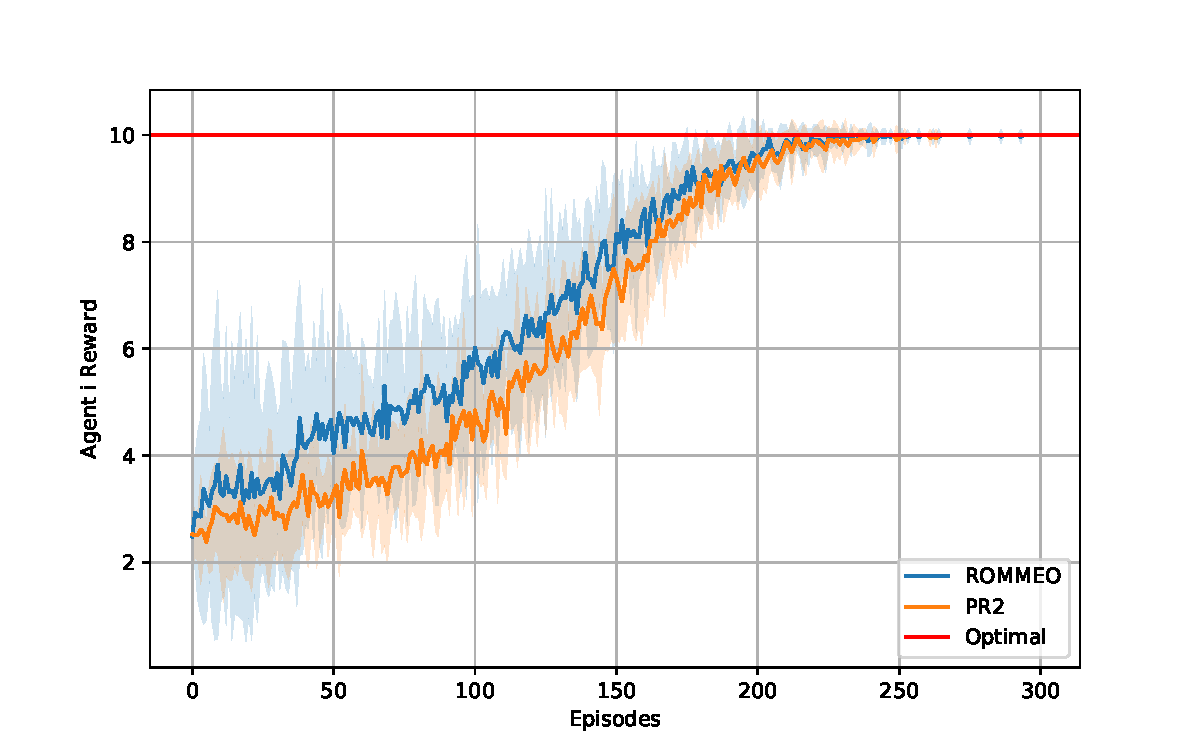
\includegraphics[scale=0.55]{figures/ROMMEO_PR2_ICG.pdf}
    \caption{The training progress of ROMMEO and PR2 on the cooperative game where the payoff is defined in equation \ref{eqn:chap3-matrix-game}.}
    \label{fig:chap3_ROMMEO_PR2}
\end{figure}
The reward of agent $j$ would be the same. We can see that ROMMEO does slightly better than PR2 as expected from the results presented in \cite{tian2019regularized}. We can see that due to the temperature schedule, the variances of both curves for the first 150 episodes are high, which is also a sign of exploration. Now, let's consider agent $i$ training when dealing with adversarial agent $j$ to study the impact of the variable $\beta^i$ and $\beta^j$ of agent $i$. We will follow the Balancing Q-learning algorithm, in which we have the following results shown in figure \ref{fig:chap3-comparison-balance-pr2-matrix}. First, in figure \ref{fig:chap3-balancing-q-min-max-matrix}, both agents converge to a Nash equilibrium when using Balancing Q-learning, which isn't the case for PR2. By misrepresentation of its opponent, agent $i$ trained under PR2 algorithm will choose action $3$ (since in cooperative case this is the best action) giving a lower reward of almost $0$ leading to suboptimal performance. On the other hand, agent $i$ that is trained under Balancing-Q will choose action $1$ yielding the reward of $2$, and reaches Nash equilibrium. 
\begin{figure}[h]
\centering
\begin{subfigure}{.5\textwidth}
  \centering
  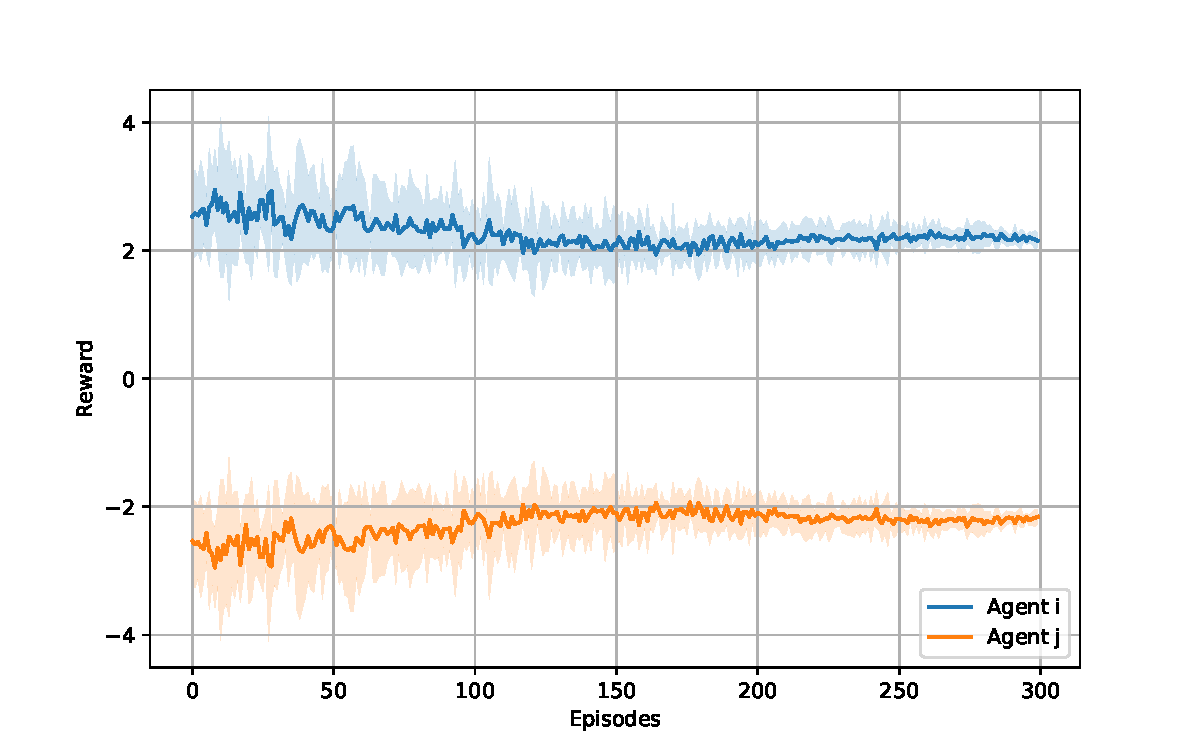
\includegraphics[width=\linewidth]{figures/Balancing_correct.pdf}
  \caption{Balancing Q-learning with adversarial opponent}
  \label{fig:chap3-balancing-q-min-max-matrix}
\end{subfigure}%
\begin{subfigure}{.5\textwidth}
  \centering
  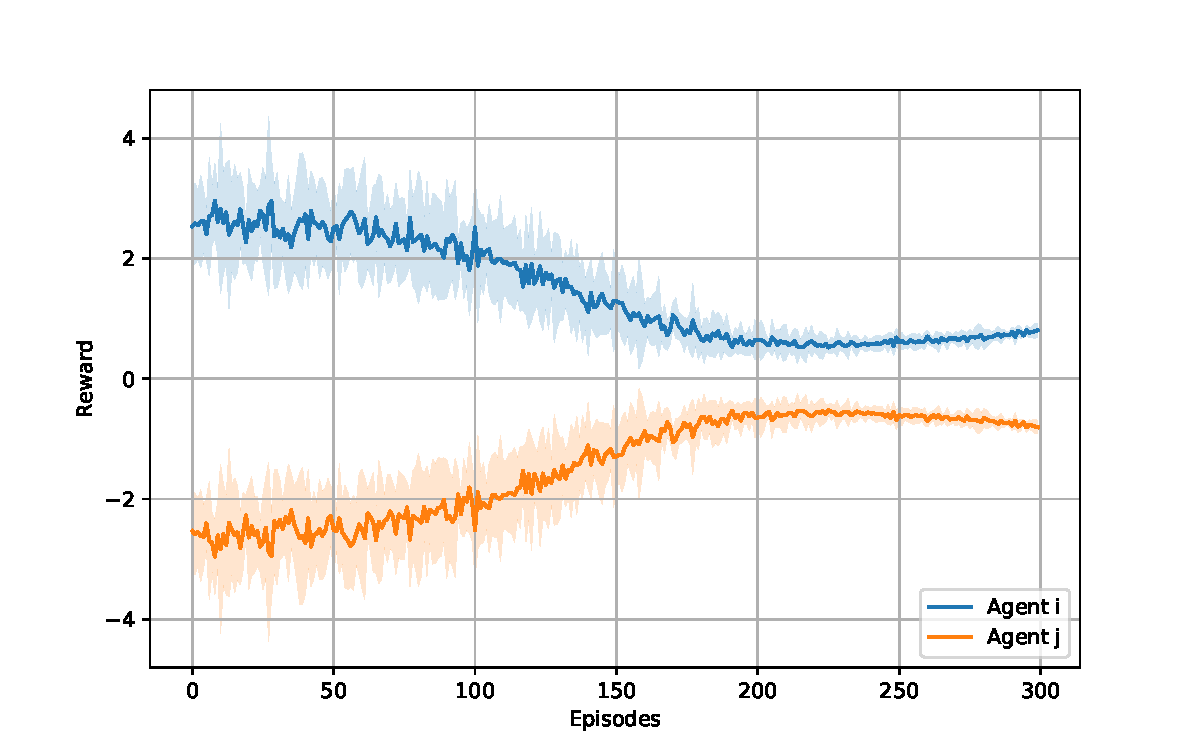
\includegraphics[width=\linewidth]{figures/Balancing_wrong.pdf}
  \caption{PR2 with misrepresentation of the opponent}
  \label{fig:chap3-pr2-min-max-matrix}
\end{subfigure}
\caption{A comparison between PR2 and Balancing Q-learning with adversarial opponent. PR2 can only represent cooperative opponent. Given the same set of seed the final reward are differ.}
\label{fig:chap3-comparison-balance-pr2-matrix}
\end{figure}

% Furthermore, one of the tricks that can be deployed to make the opponent model similar to the real opponent is to use supervised training on the prior opponent model given state and opponent action as a training set. By having a supervised opponent model, we can use it as a prior in our opponent model optimization as deployed in \cite{tian2019regularized}.

\subsection{What is Optimal ?}
We usually assume the optimality of the agent \textit{relative} to our knowledge of the opponent. If we are best responding to an optimal agent then we are likely to be optimal too\footnote{This is true in Nash equilibrium case by the definition.}. By jointly optimizing the agent with its opponent model, we can participate in what our opponent \textit{could be} given our assumptions and objective. This assumption is crucial, which will allow us to extend the framework so that it covers MAKL framework. We want to note that the assumption of an opponent's optimality is used in \cite{tian2019regularized}. However, it lacks the insight that the opponent's model doesn't have to follow the same objective as the agent, which we can show in the derivation of ROMMEO. In conclusion, MAPI is an enhanced probabilistic version of the fictitious play, where the opponent model is a fully trained policy. At the same time, the optimality of each agent should be independent while being based on each other, which is an inevitable contradiction but we will show that this is possible given special circumstances of Balancing Q-learning. 


